\section{Algoritmo exacto para el caso general}

% Para convencer a Marty, el Doc necesita mostrarle un algoritmo que
% efectivamente resuelva el problema. Dado que sus habilidades de programador
% están un poco oxidadas, se les pide diseñar e implementar un algoritmo
% exacto para MCS y desarrollar los siguientes puntos que justifiquen la
% solución encontrada:
% a) Explicar detalladamente el algoritmo implementado. Elaborar podas y
%    estrategias que permitan mejorar los tiempos de resolución.
% b) Calcular el orden de complejidad temporal de peor caso del algoritmo.
% c) Realizar una experimentación que permita observar los tiempos de
%    ejecución del algoritmo en función del tamaño de entrada y de las podas
%    y/o estrategias implementadas.

\subsection{Introducción}
En este ejercicio, se busca encontrar un algoritmo exacto para resolver, en
tiempo exponencial, el problema del \acr{MCS} entre dos grafos cualquiera.
Para ello, se utiliza la técnica de \textit{backtracking}. Este método es
extremadamente costoso tanto temporal como espacialmente, por lo que no solo
es recomendable sino necesario realizar podas y estrategias que
permitan mejorar los tiempos de resolución.

\subsection{Resolución}
El algoritmo consiste en probar todos los mapeos posibles entre los nodos de
ambos grafos, y así tomar un grafo común con la mayor cantidad de aristas de
entre todas las combinaciones de mapeos.

Dentro de la función principal, aquella que emplea la técnica de
\textit{backtracking}, se hace uso de ambos grafos, otro grafo que representa
el subgrafo común máximo dentro de la rama actual de ejecución (inicialmente
vacío), dos listas enlazadas (una para cada grafo) que contienen
los IDs de los nodos aún no mapeados en esta rama de ejecución, y un mapa
implementado sobre una tabla de \emph{hash} que contiene los mapeos hechos en esa
rama de ejecución.

\vspace{1em}

\begin{algorithm}[H]
    \SetAlgoVlined
    \caption{\acr{MCS} exacto, utilizando \emph{backtracking}}
    \label{algo:backtracking}

    \Input{Dos grafos $g_1$ y $g_2$ donde los nodos se representan con enteros,
    el subgrafo común máximo de esta rama de ejecución $mcs$ pasado por
    referencia (cada nodo en este subgrafo consiste de un par de enteros que
    representa el mapeo entre nodos de $g_1$ y $g_2$, dos listas enlazadas
    $l_1$ y $l_2$ y un mapa $mapeos$.}
    \Output{Un booleano que indica si el subgrafo pasado por referencia es
    válido (para más adelante efectuar podas).}

    \If {$l_1$.vacia() $\lor$ $l_2$.vacia()} {
        \Return{verdadero}
    }

    $maxMCS$ $\gets$ grafo de pares vacío \;

    \For {$nodo_1 \in l_1$} {
        \For {$nodo_2 \in l_2$} {

            $l_1$.borrar($nodo_1$) \;
            $l_2$.borrar($nodo_2$) \;

            $copiaMapeos$ $\gets$ $mapeos$ \;
            $copiaMapeos$.insertar($nodo_1$, $nodo_2$) \;

            $copiaMCS$ = $mcs$.clonar() \;
            $copiaMCS$.agregarNodo(par($nodo_1$, $nodo_2$)) \;

            \For {$vecino \in g_1$.vecinos($nodo_1$)} {
                $mapeadoAVecino$ $\gets$ $mapeos$.valor($vecino$) \;
                \If {$mapeos$.esta($vecino$) $\land g_2$.adyacentes($nodo_2$,
                $mapeadoAVecino$) } {
                    $copiaMCS$.agregarEje(par($nodo_1$, $nodo_2$), par($vecino$,
                    $mapeadoAVecino$))
                }
            }

            MCSBacktracking($g1$, $g2$, $copiaMCS$, $copiaMapeos$, $l_1$, $l_2$) \;

            \If {$MCSBacktraking$ es valido $\land copiaMCS$.m() $\geq maxMCS$.m()} {
                $maxMCS$ $\gets$ $copiaMCS$ \;
            }

            $l_1$.reinsertar($nodo_1$) \;
            $l_2$.reinsertar($nodo_2$) \;
        }
    }

    $mcs$ $\gets$ $maxMCS$

    \Return{verdadero}
\end{algorithm}

\vspace{1em}

Lo que se expone en el Algoritmo \ref{algo:backtracking} es el pseudocódigo
del algoritmo principal. Por simplicidad, se omiten momentáneamente las podas
del algoritmo; posteriormente se ahondará en ellas.

Se iteran $l_1$ y $l_2$
mediante dos ciclos anidados para, de esta forma, probar todos los elementos de
$l_1$ contra todos los de $l_2$ formando todos los pares de nodos posibles.
Dentro de la doble iteración se prueba el mapeo de los dos nodos seleccionados
actualizando las listas de nodos restantes y el mapa, y se hace el llamado
recursivo pasando una copia del \textit{mcs} por referencia, al cual se le
añade previamente un nodo que representa el mapeo.

Una vez terminados los ciclos se le asigna la mayor de las copias de
\textit{mcs} al subgrafo pasado por referencia.

\subsubsection{Podas y optimizaciones}

Se puede apreciar en el pseudocódigo anterior la existencia de una condición
para asignar el \textit{mcs} obtenido a la variable que almacena el máximo de
las iteraciones tras el llamado recursivo (además de la que verifica si es
su cantidad de aristas es mayor). Se pide que el resultado del llamado haya sido
válido, que es lo mismo que pedir que el valor retornado por la misma sea
verdadero. Esto podría parecer no tener sentido, ya que en todos los casos el valor
devuelto es verdadero, pero la razón de esto es que no están incluidas las podas. La
forma de podar el árbol de ejecución que utilizamos hace uso de esa condición;
si se decide cortar la rama de ejecución entonces se devuelve falso y esta
estructura evitará chequeos innecesarios.

Las podas implementadas fueron las siguientes:

\begin{enumerate}
\item Verificar que la suma de los grados de los nodos que aún no han sido
mapeados pueda ser mayor que la máxima cantidad de aristas alcanzada hasta
el momento. De no ser así, se detiene y se corta la rama que está siendo
explorada.
\item Evitar armar grafos donde las permutaciones de mapeos representan el
mismo grafo.
\end{enumerate}

La verificación de la suma de los grados es sencilla. Consiste en recorrer la
lista de nodos restantes e ir sumando los grados de cada uno de ellos. Si esa
suma junto con la cantidad de ejes del \textit{mcs} actual no puede superar
a la cantidad de ejes del máximos \textit{mcs} alcanzado en alguna de las
ramas de la ejecución previamente visitadas, entonces no tiene sentido seguir
porque no es posible llegar a una mejor solución, por lo que se corta la
ejecución.

Para esto se hace uso de una estructura condicional que termina el llamado
devolviendo falso. Esta estructura es lo primero que se ejecuta cuando se hace
el llamado recursivo. A continuación puede verse el pseudocódigo de la poda.

\begin{algorithm}
    \SetAlgoVlined
    \caption{Poda: suma de grados}
    \If {$mcs$.m() + sumaDeGrados($l_1$) $\leq$ $maximaCantEjes$} {
        \Return{falso}
    }
\end{algorithm}

$maximaCantEjes$ es una referencia a una variable que es pasada por parámetro
en el llamado recursivo y que se actualiza si se encuentra un mejor
\textit{mcs}.

La otra poda se enfoca en evitar inspeccionar una solución cuya rama de
ejecución es equivalente a una visitada anteriormente. A modo de ejemplo, sean
los grafos $A$ y $B$ con nodos $a_1, ..., a_n$ y $b_1, ..., b_k$. Durante la
ejecución del algoritmo se mapearán todas las posibles combinaciones entre
los nodos de estos grafos. Al mapearlos hay un orden que intrínsecamente
determina cual es el mejor grafo en común, es decir, según que par de nodos
se mapeen, en el siguiente llamado recursivo el mapeo de otros dos nodos
será más eficiente o no en cuestión de cantidad de aristas del \textit{mcs}.
Pero aún así, cuando el conjunto de pares de nodos mapeados es el mismo (esto
aplica para cualquier momento del algoritmo, no necesariamente tienen que
haber sido mapeados todos los nodos) puede ser permutado y el \textit{mcs}
entre los grafos será el mismo, puesto que los nodos elegidos son los mismos.
Por esto es que la intención de esta poda es evitar llegar a un grafo con el
mismo conjunto de nodos mapeados, para así ahorrar llamados.

A continuación puede verse la imagen de un ejemplo de dos grafos junto con el
árbol de mapeos que se forma, ilustrando la idea.

\begin{center}
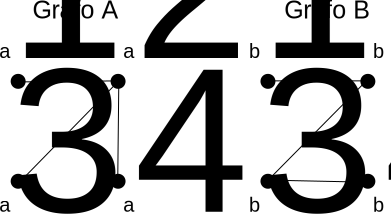
\includegraphics[width=.45\textwidth]{imagenes/ex2_grafos.pdf}
\end{center}

Las ramas en rojo son equivalentes, es decir, que representan la formación de
subgrafos comunes máximos isomorfos.

\begin{center}
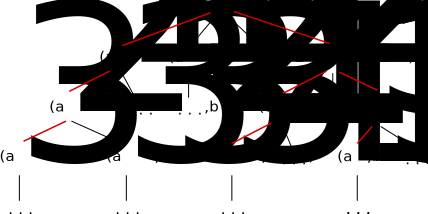
\includegraphics[width=.7\textwidth]{imagenes/ex2_execution_tree.pdf}
\end{center}

Para lograr esto utilizamos una referencia a una variable que es pasada por
parámetro en el llamado recursivo que almacena conjuntos de pares. La idea es
que antes de hacer un llamado recursivo se busque dentro de este conjunto
si el actual conjunto de mapeos ya ha sido visitado. De ser así entonces no se
hace el llamado sino que continúa la iteración, formando un nuevo par para ser
mapeado en lugar del que ha sido rechazado.

El problema con esta idea es que tiene un costo temporal demasiado alto, al
punto de representar una desventaja, ya que la comparación entre dos conjuntos
implica gran cantidad de operaciones, y esto hay que hacerlo con todos los
conjuntos de pares del mismo cardinal. A medida que la cantidad de nodos
mapeados aumenta, se vuelve más costoso, y a su vez, menos provechoso debido
a que al llegar a un nivel más profundo en la rama de ejecución, la cantidad
de llamados que pueden ser omitidos es menor.

Por esta razón, se decidió hacer efectiva esta poda únicamente para el segundo
nivel del árbol de ejecución. De esta forma las estructuras posibles se
simplifican lo suficiente como para requerir una baja complejidad temporal;
además, es el nivel en el que más ramas pueden descartarse.

La implementación de esta poda se realiza dentro del ciclo anidado, justo
después de haber elegido los nodos candidatos a ser mapeados. A continuación
puede verse el pseudocódigo de la poda.

\begin{algorithm}
    \SetAlgoVlined
    \caption{Poda: permutaciones}
    \If {$mcs$.n() == 1} {
        $permutacion$ $\gets$ tupla con el primer par mapeado y el par actual \;
        \If {$permutaciones$.esta($permutacion$)} {
            romper el ciclo \;
        }
        \Else {
            $permutaciones$.guardar($permutacion$) \;
        }
    }
\end{algorithm}

$permutaciones$ es un conjunto implementado sobre un conjunto de \emph{hash}.

La cantidad de hojas del árbol de ejecución que se ahorran es igual al
producto entre la cantidad de mapeos posibles en cada nivel, desde el tercero
hasta el último. La cantidad de mapeos posibles en un nivel es igual al
producto entre la cantidad de nodos restantes de cada grafo. Entonces, la
cantidad de hojas ahorradas es igual a $(N_1 - 2) \times (N_2 - 2) \times
(N_1 - 3) \times (N_2 - 3) \times \dots \times 1 \times (N_2 - N_1 + 1)$ si
suponemos que el segundo grafo es mayor o igual que el primero. Esto es
equivalente a $\frac{(N_1 - 2)! \times (N_2 - 2)!}{(N_2 - N_1)!}$, por lo que
fácilmente puede apreciarse por qué esta poda resulta buena.

En un principio se pensó que estas podas no resultarían demasiado efectivas,
dudando incluso de si el costo de cada una no podría significar una
desmejora en relación a la ganancia. No obstante, ambas podas no solo
acabaron siendo muy buenas, sino incluso fundamentales a medida que el tamaño de los
grafos crecía.

\subsection{Complejidad}

Para medir la complejidad del algoritmo, en principio, se analizará el
árbol de ejecución dado por el mismo. Se definen $N_1$ y $N_2$, las cantidades
de nodos de los grafos, y se supone $N_1 \leq N_2$. Por cada llamado de
la función, se hace una cantidad de llamados recursivos que depende de en qué
nivel del árbol de ejecución se encuentre actualmente el algoritmo. Esto es
así debido a que el llamado recursivo se encuentra dentro del ciclo anidado,
y la cantidad de iteraciones de ese ciclo depende de la cantidad de nodos que
aún no han sido mapeados. Como en cada llamado se mapea un par de nodos, la
cantidad de nodos por mapear va disminuyendo en cada nivel.

Para el nivel $i$ la cantidad de veces que se hace el llamado es de
$(N_1 - i)  (N_2 - i)$, que es resultado de probar todos los posibles
pares entre los nodos restantes de ambos grafos. De esta forma, la cantidad de
llamados en un nivel es de
$\frac{N_1!  N_2!}{(N_1 - i)!  (N_2 - i)!}$.

Ahora se hará foco en la complejidad del algoritmo en para cada nivel $i$.

\begin{itemize}
\item Se recorren linealmente los nodos restantes para saber si es posible
efectuar la poda de la suma de grados. $\ord(N_1 - i)$.
\item Dentro del doble ciclo anidado que se ejecuta
$(N_1 - i)  (N_2 - i)$ veces
    \begin{itemize}
    \item Copiar el mapa. $\ord(i)$.
    \item Clonar subgrafo. $\ord(i)$
    \item Agregar nodo. $\ord(i)$
    \item Agregar ejes al nuevo nodo del \acr{MCS}. Lineal sobre la cantidad de
    vecinos del nuevo nodo.
    \item Mover iteradores hasta la posición correspondiente.
    $\ord(N_1 - i + N_2 - i)$
    \end{itemize}

    Entones, el doble ciclo tiene complejidad

    \begin{align*}
    \sum_{k = 1}^{N_1 - i} \sum_{j = 1}^{N_2 - i} (\ord(i) + & \ord(\deg(v_{kj}) +
     \ord(N_1 + N_2 - 2i)) \\
    =& \sum_{k = 1}^{N_1 - i} \sum_{j = 1}^{N_2 - i} (\ord(\deg(v_{kj}) +
     \ord(N_1 + N_2)) \\
    =& \ord((N_1 - i)  (N_2 - i)  (N_1 + N_2)) + \sum_{k = 1}^{N_1 - i}
     \sum_{j = 1}^{N_2 - i} \ord(\deg(v_{kj}))
    \end{align*}

    Puede acotarse superiormente el grado de $v_{kj}$ por $N_1$, ya que no puede
    tener más de $N_1 - 1$ vecinos. Entonces, la complejidad es

    \begin{align*}
    \ord((N_1 - i) & (N_2 - i)  (N_1 + N_2)) + \sum_{k = 1}^{N_1 - i}
    \sum_{j = 1}^{N_2 - i} \ord(N_1) \\
    =& \ord((N_1 - i)  (N_2 - i)  (N_1 + N_2)) + \ord((N_1 - i)
    (N_2 - i)  N_1) \\
    =& \ord((N_1 - i)  (N_2 - i)  (N_1 + N_2 + N_1)) \\
    =& \ord((N_1 - i)  (N_2 - i)  (N_1 + N_2))
    \end{align*}

\end{itemize}

Por lo tanto la complejidad en el nivel $i$ es $\ord(N_1 - i) +$
$\ord((N_1 - i)  (N_2 - i)  (N_1 + N_2)) = \ord((N_1 - i) $
$ (N_2 - i)  (N_1 + N_2))$.

La cantidad de niveles que tiene el árbol de ejecución es $N_1$, ya que se
hacen llamados recursivos hasta que uno de los grafos tenga todos sus nodos
mapeados. Como se vio anteriormente, en cada nivel se hacen
$\frac{N_1!  N_2!}{(N_1 - i)!  (N_2 - i)!}$ llamados, por lo que
la cantidad total de llamados es de
$\sum_{i = 0}^{N_1} \frac{N_1!  N_2!}{(N_1 - i)!  (N_2 - i)!}$.

Puede acotarse esta cantidad de llamados superiormente de modo que sea
$\ord \left(N_1  \frac{N_1!  N_2!}{(N_2 - N_1)!} \right)$ siendo $N_1$ la
cantidad de niveles y $\frac{N_1!  N_2!}{(N_2 - N_1)!}$ la de hojas.

\vspace{1em}

Entonces, la complejidad total del algoritmo es

\begin{multline*}
\sum_{i = 0}^{N_1}\left[\frac{N_1!  N_2!}{(N_1 - i)!  (N_2 - i)!}
\ord((N_1 - i)  (N_2 - i)  (N_1 + N_2))\right] \\
= \ord\left(N_1  \frac{N_1!  N_2!}{(N_2 - N_1)!})
\sum_{i = 0}^{N_1}\ord((N_1 - i)  (N_2 - i)
(N_1 + N_2)\right)
\end{multline*}

Desarrollando

\[
\sum_{i = 0}^{N_1}\ord((N_1 - i)  (N_2 - i)
 (N_1 + N_2))=
(N_1 + N_2)  \sum_{i = 0}^{N_1}\ord((N_1 - i)  (N_2 - i))
\]

Sea $j = N_1 - i$ y por consecuente $i = N_1 - j$; se verifica que

\begin{align*}
\ord((N_1 + N_2)) & \sum_{i = 0}^{N_1} \ord((N_1 - i)  (N_2 - i)) \\
=& \ord((N_1 + N_2))  \sum_{j = 0}^{N_1} (\ord(j)  (N_2 - N_1 + j)) \\
=& \ord((N_1 + N_2))  \sum_{j = 0}^{N_1} (\ord(j^2) + j  (N_2 - N_1)) \\
=& \ord((N_1 + N_2))  \ord\left(\sum_{j = 0}^{N_1} j^2 + (N_2 - N_1)  \sum_{j = 0}^{N_1} j\right) \\
=& \ord((N_1 + N_2))  \ord\left(\frac{1}{6}N_1(N_1 + 1)(2N_1 + 1) + \frac{1}{2}(N_2 - N_1)N_1(N_1 + 1)\right) \\
=& \ord((N_1 + N_2))  \ord\left(\frac{1}{6}(2N_1^3 + 3N_1^2 + N_1) + \frac{1}{2}(N_2 - N_1)(N_1^2 + N_1)\right) \\
=& \ord((N_1 + N_2))  \ord\left(\frac{1}{6}(2N_1^3 + 3N_1^2 + N_1) + \frac{1}{2}(N_1^2N_2 - N_1^3 + N_1N_2 - N_1^2)\right) \\
=& \ord((N_1 + N_2))  \ord\left(\frac{1}{6}(2N_1^3 + 3N_1^2 + N_1) + \frac{1}{6}(3N_1^2N_2 - 3N_1^3 + 3N_1N_2 - 3N_1^2)\right) \\
=& \ord((N_1 + N_2))  \ord\left(\frac{1}{6}(2N_1^3 + 3N_1^2 + N_1 + 3N_1^2N_2 - 3N_1^3 + 3N_1N_2 - 3N_1^2)\right) \\
=& \ord((N_1 + N_2))  \ord\left(\frac{1}{6}(-N_1^3 + N_1 + 3N_1^2N_2 + 3N_1N_2)\right) \\
=& \ord((N_1 + N_2))  \ord\left(\frac{1}{6}N_1(-N_1^2 + 1 + 3N_1N_2 + 3N_2)\right) \\
\end{align*}

\newpage
Al verificarse que $N_1 \geq N_2$, vale que $3N_1N_2 - N_1^2 \geq 2N_1^2$.
Entonces
\begin{align*}
\ord((N_1 + N_2))  \ord\left(\frac{1}{6}N_1(-N_1^2 + 1 + 3N_1N_2 + 3N_2)\right)
=& \ord((N_1 + N_2))  \ord\left(\frac{1}{6}N_1(2N_1N_2 + 3N_2)\right) \\
=& \ord((N_1 + N_2))  \ord(N_1^2N_2) \\
=& \ord((N_1 + N_2)  N_2  N_1^2)
\end{align*}

Finalmente, la complejidad del algoritmo es
\[
\ord\left(N_1 \frac{N_1!  N_2!}{(N_2 - N_1)!}\right) \ord((N_1 + N_2)  N_2  N_1^2) =
\ord\left(\frac{N_1!  N_2!}{(N_2 - N_1)!} (N_1 + N_2)  N_2  N_1^3\right)
\]

\subsection{Experimentación}

Una vez completada la implementación del algoritmo, se realizaron pruebas
experimentales con el fin de corroborar la cota teórica calculada para la
complejidad temporal del mismo. Como fue visto anteriormente, la complejidad
del algoritmo es
$\ord\left(\frac{N_1!  N_2!}{(N_2 - N_1)!} (N_1 + N_2)  N_2  N_1^3\right)$
siempre que valga $N_1 \leq N_2$.

Entonces sólo tiene sentido experimentar para medir la complejidad siempre
que se cumpla que $N_1 \leq N_2$. Con el fin de cubrir un amplio espectro de
la región acotada por esta condición se formularon experimentos que emplean
distintos valores para las cantidades de nodos de los grafos en cuestión.

\begin{enumerate}[label=\alph*)]
\item $N_1 = N_2$
\item $2N_1 = N_2$
\item $N_1 = C$
\end{enumerate}

A continuación se analiza la complejidad del algoritmo considerando las
cantidades de nodos descriptas previamente:

\begin{enumerate}[label=\alph*.]
\item
$\ord\left(\frac{N_1!  N_2!}{(N_2 - N_1)!} (N_1 + N_2)  N_2  N_1^3\right)$
$=\ord((N_1!)^2 N_1^5)$

\item
$\ord\left(\frac{N_1!  N_2!}{(N_2 - N_1)!} (N_1 + N_2)  N_2  N_1^3\right)$
$=\ord\left(\frac{N_1! (2N_1)!}{(2N_1 - N_1)!} (N_1 + 2N_1)  2N_1  N_1^3\right)$

\ \ \ \ \ \ \ \ \ \ \ \ \ \ \ \ \ \ \ \ \ \ \ \ \ \ \ \ \ \ \ \ \ \ \ \ \ \ \ \ 
$=\ord\left(\frac{N_1! (2N_1)!}{(N_1)!} 3N_1 2N_1  N_1^3\right)$

\ \ \ \ \ \ \ \ \ \ \ \ \ \ \ \ \ \ \ \ \ \ \ \ \ \ \ \ \ \ \ \ \ \ \ \ \ \ \ \ 
$=\ord\left((2N_1)! N_1^5\right)$

\item
$\ord\left(\frac{N_1!  N_2!}{(N_2 - N_1)!} (N_1 + N_2)  N_2  N_1^3\right)$
$=\ord\left(\frac{C! N_2!}{(N_2 - C)!} (C + N_2)  N_2  C^3\right)$

\ \ \ \ \ \ \ \ \ \ \ \ \ \ \ \ \ \ \ \ \ \ \ \ \ \ \ \ \ \ \ \ \ \ \ \ \ \ \ \ 
$=\ord\left(\frac{N_2!}{(N_2 - C)!}N_2^2\right)$
\end{enumerate}

Para evitar la interferencia en las mediciones de la morfología del grafo, se
fijó cada experimento para una familia de grafos determinada. Así, se tiene un
mayor control de las variables involucradas. Sin embargo, para verificar que
la cota teórica de complejidad no se cumple de forma accidental, sino que vale
para grafos de cualquier tipo, se probó con varias familias distintas.

Se experimento con las siguientes familias de grafos:

\begin{itemize}
\item \textit{Completos}: Grafo completo vs. grafo completo
\item \textit{Árboles}: Árbol vs. árbol
\item \textit{Ciclos}: Ciclos simple vs. ciclo simple
\item \textit{Bipartitos}: Grafo bipartito completo vs. grafo bipartito
completo
\end{itemize}

Se exponen ahora los gráficos de los resultados de las experimentaciones. Se
exhibe uno por cada relación en la cantidad de nodos de los grafos utilizados
distinta. Para cada uno de ellos se grafican los datos obtenidos de cada una
de las familias de grafos ya mencionadas junto a la cota de complejidad
calculada para cada caso, para así compararlas y poder observar que para cada
una de ellas el algoritmo cumple con la cota de complejidad calculada.

Las cotas de complejidad son multiplicadas por una constante que ajusta su
valor al de las experimentaciones como mas conveninete sea para poder apreciar
con mayor facilidad si el algoritmo cumple o no con ellas.

\newcommand\constante{1}
En la Figura \ref{fig:exp2:n_1_eq_n_2} pueden observarse los datos obtenidos
de la experimentación en el caso en que $N_1 = N_2$.

\begin{figure}[H]
    \caption{Tiempos de ejecución observados para $N_1 = N_2$.}
    \label{fig:exp2:n_1_eq_n_2}
    \centering
    \begin{tikzpicture}
        \begin{axis}[
                title={},
                xlabel={Cantidad de nodos ($N_1$)},
                ylabel={Tiempo de ejecución (nanosegundos)},
                scaled x ticks=false,
                scaled y ticks=false,
                enlargelimits=0.05,
                width=0.5\textwidth,
                height=0.5\textwidth,
                legend pos=outer north east,
                legend cell align=left,
                ymode=log
            ]
            \addplot[color=black] table[x index=0,y expr={\constante * x! * x! * x^5}]{../exp/ej2/equal_complete_vs_complete};
            \addplot[color=orange] table[x index=0,y index=1]{../exp/ej2/equal_complete_vs_complete};
            \addplot[color=blue] table[x index=0,y index=1]{../exp/ej2/equal_tree_vs_tree};
            \addplot[color=red] table[x index=0,y index=1]{../exp/ej2/equal_cycle_vs_cycle};
            \addplot[color=green] table[x index=0,y index=1]{../exp/ej2/equal_complete_bipartite_vs_complete_bipartite};

            \legend{
                $(N_1!)^2 N_1^5$,
                \textit{Completos},
                \textit{Árboles},
                \textit{Ciclos},
                \textit{Bipartitos}
            }
        \end{axis}
    \end{tikzpicture}
\end{figure}

Con la intención de lograr una mejor comparativa de los tiempos de ejecución
de cada familia de grafos con la cota de complejidad se analiza un cociente
entre cada familia y dicha cota. En la Figura
\ref{fig:exp2:n_1_eq_n_2:cociente} puede observarse este cociente, en donde se
grafica también la constante utilizada para ajustar la cota de complejidad,
que en este caso es 1.

\begin{figure}[H]
    \caption{Cociente entre los tiempos de ejecución observados para $N_1 = N_2$ y su cota de complejidad.}
    \label{fig:exp2:n_1_eq_n_2:cociente}
    \centering
    \begin{tikzpicture}
        \begin{axis}[
                title={},
                xlabel={Cantidad de nodos ($N_1$)},
                ylabel={Tiempo de ejecución (nanosegundos) / $\left((N_1!)^2 N_1^5\right)$},
                scaled x ticks=false,
                scaled y ticks=false,
                enlargelimits=0.05,
                width=0.5\textwidth,
                height=0.5\textwidth,
                legend pos=outer north east,
                legend cell align=left,
                ymode=log
            ]
            \addplot[color=black] table[x index=0,y expr={\constante}]{../exp/ej2/equal_complete_vs_complete};
            \addplot[color=orange] table[x index=0,y expr={\thisrowno{1} / (x! * x! * x^5)}]{../exp/ej2/equal_complete_vs_complete};
            \addplot[color=blue] table[x index=0,y expr={\thisrowno{1} / (x! * x! * x^5)}]{../exp/ej2/equal_tree_vs_tree};
            \addplot[color=red] table[x index=0,y expr={\thisrowno{1} / (x! * x! * x^5)}]{../exp/ej2/equal_cycle_vs_cycle};
            \addplot[color=green] table[x index=0,y expr={\thisrowno{1} / (x! * x! * x^5)}]{../exp/ej2/equal_complete_bipartite_vs_complete_bipartite};

            \legend{
                $\constante$,
                $\frac{\textit{Completos}}{(N_1!)^2 N_1^5}$,
                $\frac{\textit{Árboles}}{(N_1!)^2 N_1^5}$,
                $\frac{\textit{Ciclos}}{(N_1!)^2 N_1^5}$,
                $\frac{\textit{Bipartitos}}{(N_1!)^2 N_1^5}$
            }
        \end{axis}
    \end{tikzpicture}
\end{figure}

Es notorio como cada una de las familias de grafos utilizadas para esta
experimentación permanecen por debajo de la constante, lo cual indica entonces
que para el caso en que $N_1 = N_2$ el algoritmo cumple con la cota de
complejidad calculada, que es de orden $(N_1!)^2 N_1^5$, para cada una de
estas familias.

\renewcommand\constante{1}
Se expone ahora, en la Figura \ref{fig:exp2:2n_1_eq_n_2}, un gráfico con los
datos obtenidos de la experimentación en el caso en que $2N_1 = N_2$, junto a
la cota de complejidad para este caso que es $\ord((2N_1)! N_1^5)$.

\begin{figure}[H]
    \caption{Tiempos de ejecución observados para $2N_1 = N_2$.}
    \label{fig:exp2:2n_1_eq_n_2}
    \centering
    \begin{tikzpicture}
        \begin{axis}[
                title={},
                xlabel={Cantidad de nodos ($N_2$)},
                ylabel={Tiempo de ejecución (nanosegundos)},
                scaled x ticks=false,
                scaled y ticks=false,
                enlargelimits=0.05,
                width=0.5\textwidth,
                height=0.5\textwidth,
                legend pos=outer north east,
                legend cell align=left,
                ymode=log
            ]
            \addplot[color=black] table[x index=0,y expr={\constante * ((2 * x)! * x^5}]{../exp/ej2/lineal_complete_vs_complete};
            \addplot[color=orange] table[x index=0,y index=1]{../exp/ej2/lineal_complete_vs_complete};
            \addplot[color=blue] table[x index=0,y index=1]{../exp/ej2/lineal_tree_vs_tree};
            \addplot[color=red] table[x index=0,y index=1]{../exp/ej2/lineal_cycle_vs_cycle};
            \addplot[color=green] table[x index=0,y index=1]{../exp/ej2/lineal_complete_bipartite_vs_complete_bipartite};

            \legend{
                $(2N_1)! N_1^5$,
                \textit{Completos},
                \textit{Árboles},
                \textit{Ciclos},
                \textit{Bipartitos}
            }
        \end{axis}
    \end{tikzpicture}
\end{figure}

Al igual que en el experimento anterior, se grafica en la Figura
\ref{fig:exp2:2n_1_eq_n_2:cociente} el cociente entre los datos obtenidos y la
cota de complejidad de la experimentación para el caso en que $2N_1 = N_2$,
junto con la constante que multiplica la función descripta por la cota de
complejidad que en este caso es \constante.

\begin{figure}[H]
    \caption{Cociente entre los tiempos de ejecución observados para $2N_1 = N_2$ y su cota de complejidad.}
    \label{fig:exp2:2n_1_eq_n_2:cociente}
    \centering
    \begin{tikzpicture}
        \begin{axis}[
                title={},
                xlabel={Cantidad de nodos ($N_2$)},
                ylabel={Tiempo de ejecución (nanosegundos) / $((2N_1)! N_1^5)$},
                scaled x ticks=false,
                scaled y ticks=false,
                enlargelimits=0.05,
                width=0.5\textwidth,
                height=0.5\textwidth,
                legend pos=outer north east,
                legend cell align=left,
                ymode=log
            ]
            \addplot[color=black] table[x index=0,y expr={\constante}]{../exp/ej2/lineal_complete_vs_complete};
            \addplot[color=orange] table[x index=0,y expr={\thisrowno{1} / ((2 * x)! * x^5)}]{../exp/ej2/lineal_complete_vs_complete};
            \addplot[color=blue] table[x index=0,y expr={\thisrowno{1} / ((2 * x)! * x^5)}]{../exp/ej2/lineal_tree_vs_tree};
            \addplot[color=red] table[x index=0,y expr={\thisrowno{1} / ((2 * x)! * x^5)}]{../exp/ej2/lineal_cycle_vs_cycle};
            \addplot[color=green] table[x index=0,y expr={\thisrowno{1} / ((2 * x)! * x^5)}]{../exp/ej2/lineal_complete_bipartite_vs_complete_bipartite};

            \legend{
                $\constante$,
                $\frac{\textit{Completos}}{(2N_1)! N_1^5}$,
                $\frac{\textit{Árboles}}{(2N_1)! N_1^5}$,
                $\frac{\textit{Ciclos}}{(2N_1)! N_1^5}$,
                $\frac{\textit{Bipartitos}}{(2N_1)! N_1^5}$
            }
        \end{axis}
    \end{tikzpicture}
\end{figure}

Al igual que en el caso anterior, puede observarse como cada una de las
familias de grafos empleadas en esta experimentación permanecen por debajo de
la constante, lo cual indica entonces que para el caso en que $2N_1 = N_2$ el
algoritmo cumple con la cota de complejidad calculada de orden $(2N_1)! N_1^5$,
para cada una de estas familias.

\renewcommand\constante{5000}
\newcommand\valorFijo{4}
Finalmente, en la Figura \ref{fig:exp2:n_1_eq_fijo} pueden verse los datos
obtenidos de la experimentación en el caso en que $N_1 = C$. El valor elegido
es $C = \valorFijo$.

La razón por la cual el valor en que $C$ fue fijado sea \valorFijo es que para
valores muy chicos el algoritmo no ejecutaba demasiadas operaciones, lo cual
no hubiese sido fructuosa a raíz de la experimentación, y para valores grandes
el tiempo de ejecución es muy alto, lo suficiente como para correr durante
días. Como existe la condición de que $N_1 \leq N_2$, si se fija para $C$ un
valor muy alto, el algoritmo debera efectuar la búsqueda para un grafo con una
cantidad alta de nodos y otro con una cantidad mayor aún. Para un numero de 8
nodos por grafo el algoritmo comienza a enlentecerse mucho, entonces
se estableció $C = 4$ ya que permite una experimentación de tiempo aceptable,
y además un rango de nodos suficiente como para considerar la experimentación
representativa para valores mayores.

\begin{figure}[H]
    \caption{Tiempos de ejecución observados para $N_1 = \valorFijo$.}
    \label{fig:exp2:n_1_eq_fijo}
    \centering
    \begin{tikzpicture}
        \begin{axis}[
                title={},
                xlabel={Cantidad de nodos ($N_2$)},
                ylabel={Tiempo de ejecución (nanosegundos)},
                scaled x ticks=false,
                scaled y ticks=false,
                enlargelimits=0.05,
                width=0.5\textwidth,
                height=0.5\textwidth,
                legend pos=outer north east,
                legend cell align=left,
                ymode=log
            ]
            \addplot[color=black] table[x index=0,y expr={\constante * x! / (x - \valorFijo)! * x^2}]{../exp/ej2/fixed_complete_vs_complete};
            \addplot[color=orange] table[x index=0,y index=1]{../exp/ej2/fixed_complete_vs_complete};
            \addplot[color=blue] table[x index=0,y index=1]{../exp/ej2/fixed_tree_vs_tree};
            \addplot[color=red] table[x index=0,y index=1]{../exp/ej2/fixed_cycle_vs_cycle};
            \addplot[color=green] table[x index=0,y index=1]{../exp/ej2/fixed_complete_bipartite_vs_complete_bipartite};

            \legend{
                $\constante \frac{N_2!}{(N_2 - \valorFijo)!}N_2^2$,
                \textit{Completos},
                \textit{Árboles},
                \textit{Ciclos},
                \textit{Bipartitos}
            }
        \end{axis}
    \end{tikzpicture}
\end{figure}

Al igual que en el experimento anterior, se grafica en la Figura
\ref{fig:exp2:2n_1_eq_n_2:cociente} el cociente entre los datos obtenidos y la
cota de complejidad de la experimentación para el caso en que $2N_1 = N_2$,
junto con la constante que multiplica la función descripta por la cota de
complejidad que en este caso es \constante.
En la Figura \ref{fig:exp2:n_1_eq_fijo:cociente} puede verse el cociente entre
los datos obtenidos y la cota de complejidad de la experimentación en el caso
en que $N_1 = C$, siendo $C = \valorFijo$. También se grafica la constante que
multiplica la función descripta por la cota de complejidad que en este caso es
\constante.

\begin{figure}[H]
    \caption{Cociente entre los tiempos de ejecución observados para $N_1 = \valorFijo$ y su cota de complejidad.}
    \label{fig:exp2:n_1_eq_fijo:cociente}
    \centering
    \begin{tikzpicture}
        \begin{axis}[
                title={},
                xlabel={Cantidad de nodos ($N_2$)},
                ylabel={Tiempo de ejecución (nanosegundos) / $\left(\frac{N_2!}{(N_2 - \valorFijo)!}N_2^2\right)$},
                scaled x ticks=false,
                scaled y ticks=false,
                enlargelimits=0.05,
                width=0.5\textwidth,
                height=0.5\textwidth,
                legend pos=outer north east,
                legend cell align=left,
                ymode=log,
                xmin=4
            ]
            \addplot[color=black] table[x index=0,y expr={\constante}]{../exp/ej2/fixed_complete_vs_complete};
            \addplot[color=orange] table[x index=0,y expr={\thisrowno{1} / (x! / (x - \valorFijo)! * x^2)}]{../exp/ej2/fixed_complete_vs_complete};
            \addplot[color=blue] table[x index=0,y expr={\thisrowno{1} / (x! / (x - \valorFijo)! * x^2)}]{../exp/ej2/fixed_tree_vs_tree};
            \addplot[color=red] table[x index=0,y expr={\thisrowno{1} / (x! / (x - \valorFijo)! * x^2)}]{../exp/ej2/fixed_cycle_vs_cycle};
            \addplot[color=green] table[x index=0,y expr={\thisrowno{1} / (x! / (x - \valorFijo)! * x^2)}]{../exp/ej2/fixed_complete_bipartite_vs_complete_bipartite};

            \legend{
                $\constante$,
                \textit{Completos}$\frac{(N_2 - \valorFijo)!}{N_2! N_2^2}$,
                \textit{Árboles}$\frac{(N_2 - \valorFijo)!}{N_2! N_2^2}$,
                \textit{Ciclos}$\frac{(N_2 - \valorFijo)!}{N_2! N_2^2}$,
                \textit{Bipartitos}$\frac{(N_2 - \valorFijo)!}{N_2! N_2^2}$
            }
        \end{axis}
    \end{tikzpicture}
\end{figure}

Al observar que el algoritmo permanece por debajo de la constante para todas
las familias de grafos con las que se experimentó, se puede apreciar que
cumple con la cota de complejidad calculada para el caso en que se fija
$N_1 = C$.

\subsection{Conclusión}

Una vez finalizadas las experimentaciones para los casos expuestos se llegó a
la conclusión de que el algoritmo cumple con la complejidad calculada, en
vista de que las combinaciones de casos y familias de grafos planteadas cubren
una buena cantidad de instancias, en cada caso se desempeña en un tiempo menor
a la cota de complejidad calculada, y que se lo considera representativo para
instancias mayores a las expuestas dentro del rango de la muestra.

Una observación adicional surgida de la experimentación es que para grafos
completos los tiempos de ejecución del algoritmo se alejan (son bastante
mayores) del resto de las familias de grafos empleadas en los experimentos.
Esto tiene sentido ya que al haber una mucho mayor densidad de aristas que en
el resto de los casos, generalmente el grado de los nodos en es mucho mayor,
lo cual implica una mayor cantidad de operaciones al momento de verificar
las vecindades de los distintos nodos que se tienen en cuenta a lo largo de la
ejecución del algoritmo.